\section*{Dati e risultati}

\subsection*{Circuito invertente}

Il primo circuito studiato sfrutta l'opamp LM741 al fine di amplificare e sfasare di $180^\circ$ il segnale in ingresso ($V\ped{in}$). Il circuito che abbiamo realizzato è illustrato in Figura \ref{fig:amp_inv}.
Questo circuito è alimentato con una tensione costante positiva di $\SI{+15}{\volt}$ e una negativa di $\SI{-15}{\volt}$.
Abbiamo collegato in ingresso un segnale sinusoidale ($V\ped{in}$) ottenuto grazie al generatore di onde.

Dal momento che vogliamo che tale circuito abbia un guadagno ($G$) di circa 10 dobbiamo dimensionarlo. In particolare, facendo l'analisi circuitale si ottiene che vale la relazione:

\begin{equation}
        G\,=\,-\frac{V\ped{out}}{V\ped{in}}\,=\,-\frac{R_2}{R_1} \qquad \implies \qquad |R_2|\,=\,10\,|R_1|
        \label{eq:g}
\end{equation}
%
dove $R_1$ e $R_2$ sono le resistenze riportate in figura, $V\ped{in}$ il segnale in ingresso e $V\ped{out}$ il segnale in uscita. Quindi, per non avere correnti troppo elevate all'interno del circuito (che dissiperebbero energia), abbiamo deciso di porre $R_2\,=\,\SI{100}{\kilo\ohm}$ e $R_1\,=\,\SI{10}{\kilo\ohm}$.

È stato quindi verificato che il guadagno di tale circuito, a frequenza fissta $\nu\,=\,\SI{1}{\kilo\hertz}$, fosse costante. A tal fine abbiamo misurato $V\ped{out}$ al variare dell'ampiezza del segnale in ingresso $V\ped{in}$. Poichè il guadagno è circa costante al variare dell'ampiezza, sfruttando la relazione (\ref{eq:g}) abbiamo fatto la media dei valori di $G$ così ricavati e abbiamo ottenuto che il guadagno del nostro circuito vale:

\begin{equation}
        G\,=\, 9.80 \pm 0.05
\end{equation}

Successivamente abbiamo deciso di studiare come varia il guadagno al variare della frequenza di $V\ped{in}$, mantenendo costante l'ampiezza $V\ped{in}$ a 515 mV picco-picco. Quello che abbiamo ottenuto è riportato in Figura \ref{fig:g_vs_freq}.

\begin{SCfigure}
    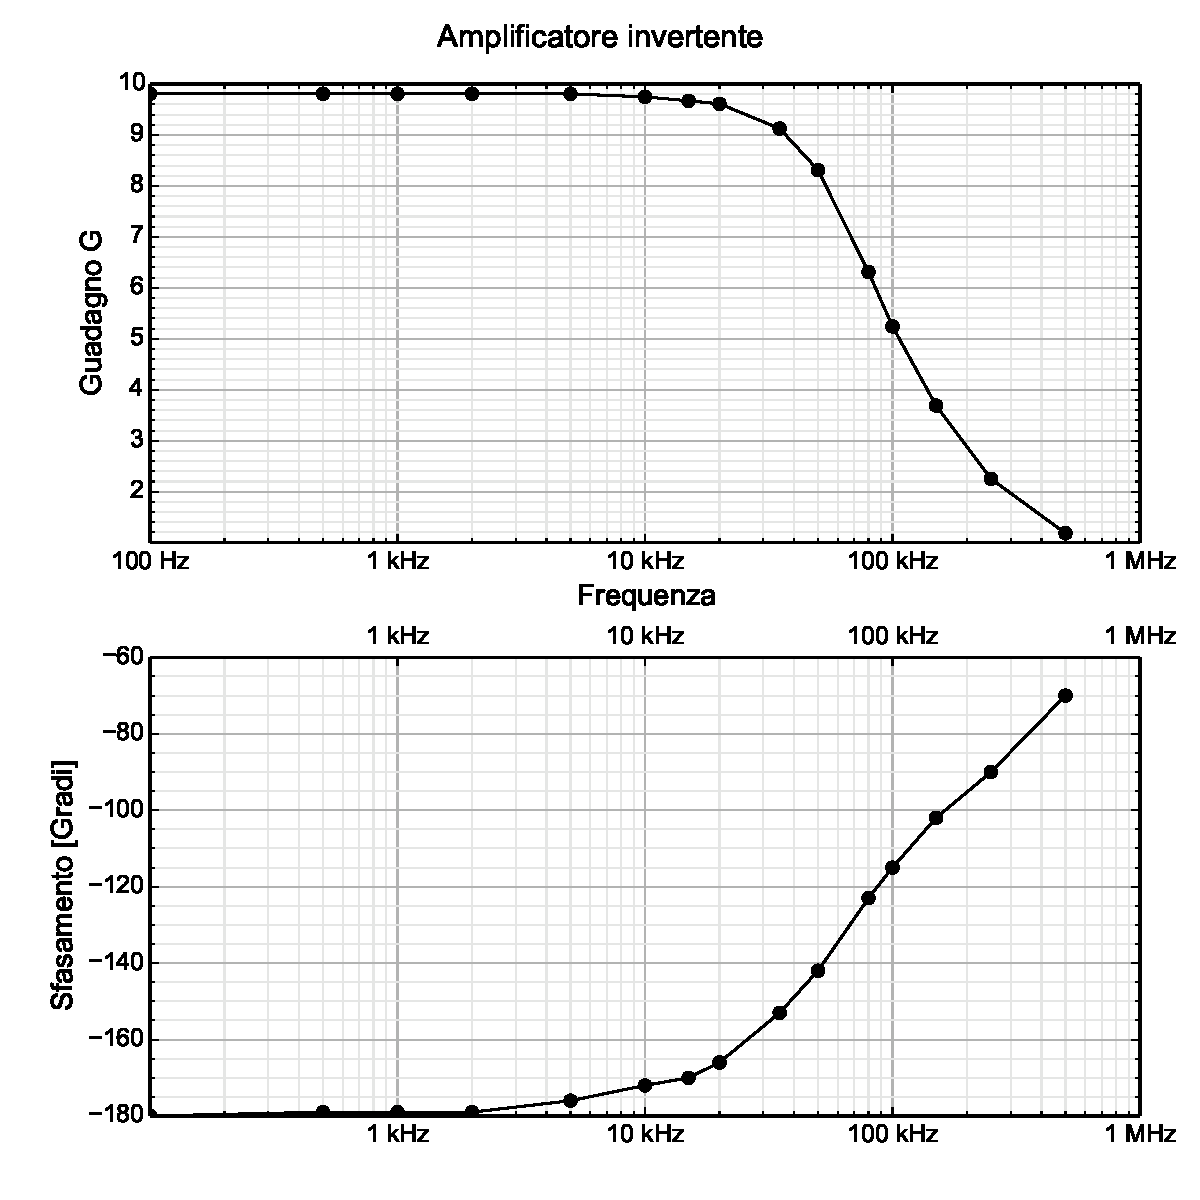
\includegraphics[width=0.75\textwidth]{amp_inv.pdf}
    \caption{La figura mostra gli andamenti di guadagno e sfasamento in funzione della
        frequenza dell'onda sinusoidale in ingresso per il circuito \ref{fig:amp_inv}. L'ampiezza del segnale è
        stata mantenuta costante a 515 mV picco-picco. Le barre d'errore non sono riportate percè simili alla dimensione
        dei punti. Tra i 10 kHz e i 20 kHz il segnale il circuito inizia a tagliare. Il punto -3dB è a circa a 100 kHz.
        Inoltre il circuito sfasa anche l'uscita e lo sfasamento varia con la frequenza, anche se non è proprio di 90$^\circ$
        a 100 kHz, ma circa 110$^\circ$. Il circuito si comporta come un filtro passa-basso ed è quindi adatto ad essere usato
        per basse frequenze.}
    \label{fig:g_vs_freq}
\end{SCfigure}

Infine abbiamo trovato i valori di ampiezza del segnale in uscita $V\ped{out}$, a frequenza costante $\nu\,=\,\SI{1}{\kilo\hertz}$ di $V\ped{in}$, per i quali si verifica il fenomeno del clamping. Tali valori sono risultati essere:

\begin{equation}
        V\ped{out}^{+}\,\simeq\,\SI{14.2}{\volt} \qquad \text{e} \qquad V\ped{out}^{-}\,\simeq\,\SI{-13.1}{\volt}
        \label{eq:clamping_1}
\end{equation}

\subsection*{Circuito non invertente}

Questo circuito, come il precedente, sfrutta l'op-amp LM741 al fine di ottenere un'amplificazione del segnale in ingresso $V\ped{in}$, ma in questo caso non è presente uno sfasamento di $180^\circ$ tra i due segnali ($V\ped{in}$ e $V\ped{out}$).
Il circuito utilizzato è riportato in Figura \ref{fig:amp_noninv}. Le sue specifiche sono esattamente uguali a quelle del circuito descritto in precedenza a parte il fatto che le due resistenze $R_1$ e $R_2$ sono posizionate in punti differenti del circuito.

Anche in questo caso abbiamo svolto delle misure di $V\ped{out}$ in funzione di $V\ped{in}$, mantenedo costante la frequenza $\nu\,=\,\SI{1}{\kilo\hertz}$ di $V\ped{in}$. Dall'analisi del circuito risulta che 

\begin{equation}
    G \,=\, 1 + \frac{R_2}{R_1} = 10.66 \pm 0.06
\end{equation}
%
dove il valore numerico è la media dei valori che abbiamo ottenuto per diverse ampiezze di $V\ped{in}$.

Successivamente abbiamo valutato l'andamento di $V\ped{out}$ in funzione della frequenza di $V\ped{in}$, tenendo fissa
l'ampiezza del segnale in ingresso a 519 mV, e abbiamo ottenuto quanto illustrato in Figura \ref{fig:g2}.

\begin{SCfigure}
    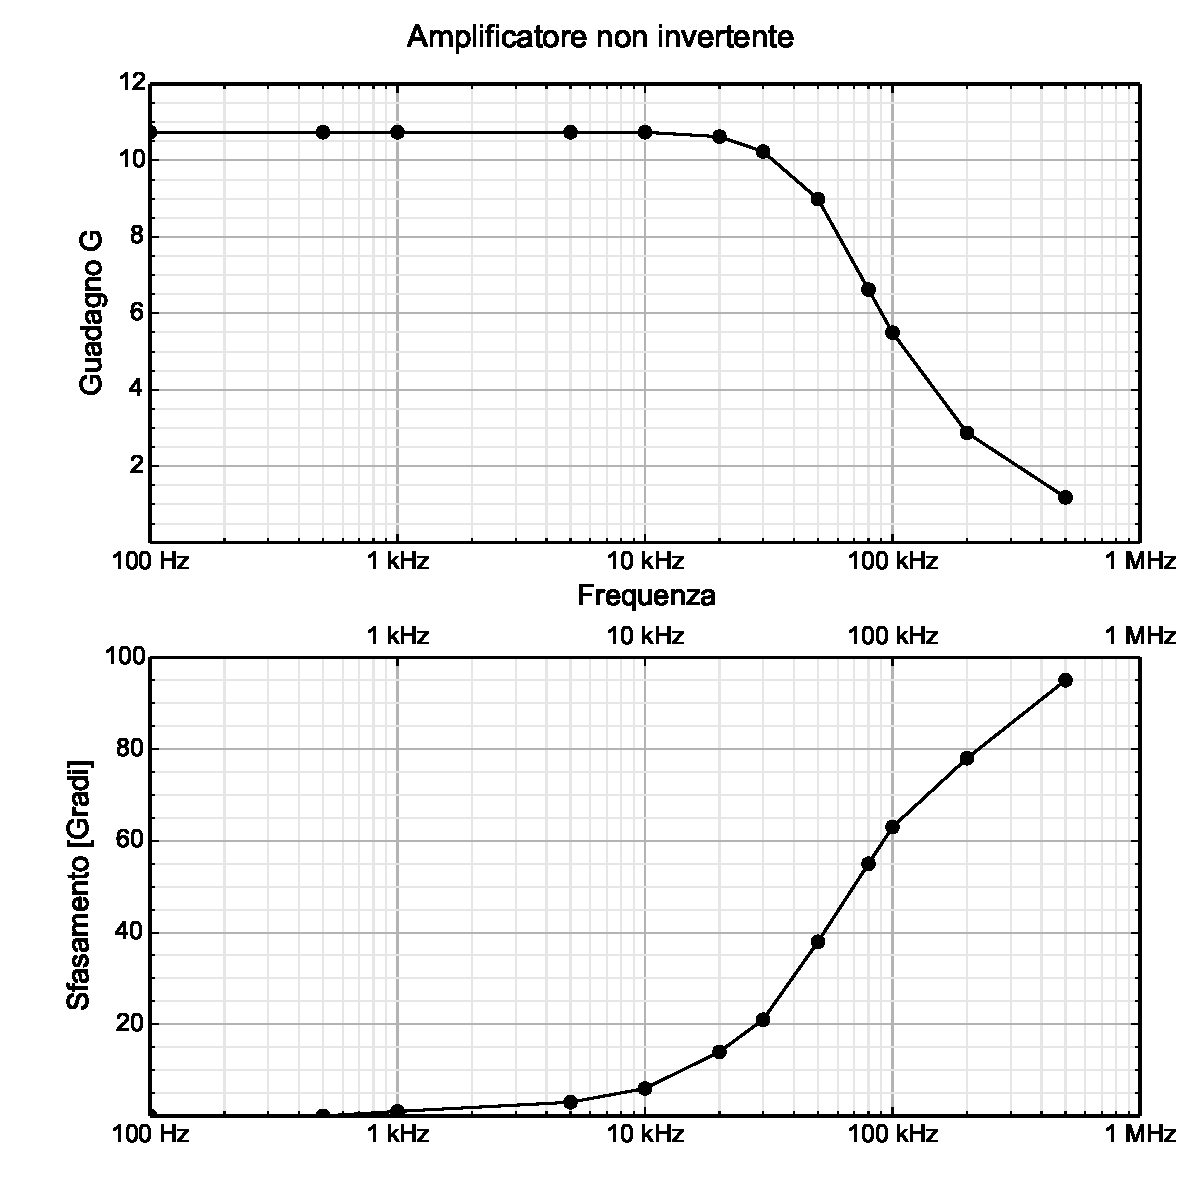
\includegraphics[width=0.75\textwidth]{amp_ninv.pdf}
    \caption{La figura mostra gli andamenti di guadagno e sfasamento in funzione della
        frequenza dell'onda sinusoidale in ingresso per il circuito \ref{fig:amp_ninv}. L'ampiezza del segnale è
        stata mantenuta costante a 519 mV picco-picco. Le barre d'errore non sono riportate percè simili alla dimensione
        dei punti. Anche in questo caso il circuito si comporta come un passa basso, con frequenza di taglio
        (-3dB) a circa a 100 kHz. La degradazione del guadagno comincia tra i 20 kHz e i 30 kHz.
        Lo sfasamento varia con la frequenza e a 100 kHz è di circa 65$^\circ$.}
    \label{fig:g2}
\end{SCfigure}

Infine, come nell'analisi dl circuito precedente, abbiamo trovato i valori di ampiezza del segnale in uscita $V\ped{out}$, a frequenza costante $\nu\,=\,\SI{1}{\kilo\hertz}$ di $V\ped{in}$, per i quali si verifica il fenomeno del clamping. Tali valori sono risultati essere:

\begin{equation}
        V\ped{out}^+\,\simeq\,\SI{13.2}{\volt} \qquad \text{e} \qquad V\ped{out}^-\,\simeq\,\SI{-13.1}{\volt}
\end{equation}

\subsection*{Circuito sommatore}

Come passo successivo abbiamo utilizzato il nostro amplificatore operazionale per realizzare un circuito sommatore, rappresentato in Figura \ref{fig:sum}. Questo circuito ha lo scopo di ricevere in ingresso più segnali $V_i$ e di restituire in output la loro somma pesata sui relativi valori di $R_i$. In formule:

\begin{equation}
        V\ped{out}\,=\,-\sum_{i=1}^{n}{\frac{R}{R_i} \cdot V_i}
        \label{eq:summa}
\end{equation}
%
dove $R$ è il valore di resistenza della retroazione, $V_i$ sono i vari valori di tensione in ingresso e $R_i$ i valori di resistenze dell'input corrispondente. Si noti il segno meno, che implica che la somma dei valori viene anche ribaltata, fatto
che può portare a confusione se non è sottolineato a dovere.

Come è facile notare, nel nostro caso, ci sono solo due valori di $V_i$ ovvero $V_1$ e $V_2$ e $R_1$, $R_2$ ed $R$ hanno lo stesso valore di $\SI{10}{\kilo\ohm}$. Inoltre il segnale $V_1$ è fornito dal generatore d'onde, quindi ne potevamo variare l'ampiezza e la frequenza, mentre il segnale $V_2$ è ottenuto grazie alla sorgente di tensione alternata, di fequenza $\nu_0\,=\,\SI{50}{\hertz}$, con un'ampiezza picco-picco di $\SI{15}{\volt}$. Anche in questo caso l'amplificatore operazionale è alimentato tra una tensione posistiva di $\SI{+15}{\volt}$ e una negativa di $\SI{-15}{\volt}$.

Pertanto una volta montato il circuito ci siamo serviti dell'oscilloscopio per verificare che effettivamente quello che abbiamo realizzato fosse un circuito sommatore. Il risultato ottenuto è riportato in Figura \ref{fig:sums}.

\begin{figure}[h]
    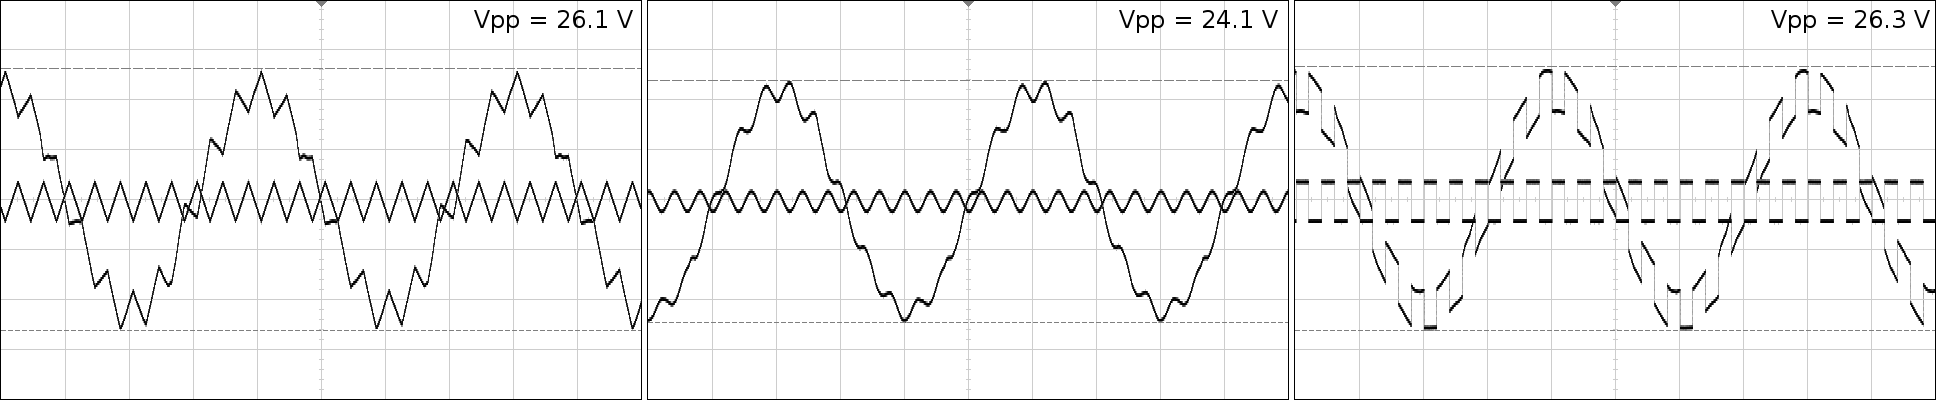
\includegraphics[width=\textwidth]{sum.png}
    \caption{La figura illustra il funzionamento del circuito sommatore. In input sono stati collegati un alimentatore che
        fornisce un segnale sinusoidale 15 V picco-picco a 50 Hz (non mostrato in figura) e
        il generatore di funzioni d'onda, che abbiamo impostato per fornire segnali di ampiezza
        4.2 V picco-picco a 500 Hz (onde piccole nelle figure). Nella prima figura abbiamo usate il generatore
        per fornire un segnale a dente di sega,
        nel secondo una sinusoide e nel terzo un onda quadra. L'output sono le tre curve grandi nelle figure. Può sembrare che
        il circuito sottragga invece di sommare, ma bisogna considerare il segno meno nella formula \eqref{eq:summa}.
        L'onda fornita dall'alimentatore è sfasata di 180$^\circ$ rispetto alla componente principale dell'output. Considerando
        questo fatto, si vede che il circuito somma e poi inverte il segnale. Ogni quadretto sono 5 V.
        }
    \label{fig:sums}
\end{figure}

\subsection*{Circuito integratore}

In questa sezione della relazione ci occupiamo di studiare le caratteristiche del circuito illustrato in Figura \ref{fig:int} realizzato con il solito op-amp LM741.

Le specifiche del circuito sono riportate in Figura \ref{fig:int}, tuttavia facciamo notare che in ingresso $V\ped{in}$ è stato applicato un segnale variabile nel tempo sfruttando il generatore di onde. Inoltre si noti che la resistenza $R_2$ del ramo di
retroazione serve a fornire un passaggio per la corrente a basse frequenze, in modo che l'integratore non vada in saturazione.
 
Lo scopo di questo circuito, idealmente, è quello di fornire un segnale in uscita $V\ped{out}$ che,
come dice il nome stesso, è l'integrale del segnale in ingesso $V\ped{in}$. Ovvero matematicamente:

\begin{equation}
    V\ped{out}\,=\,-\frac{1}{R_1C} \int_{t}{V\ped{in}(t) \, dt}\,+\,c
\end{equation}
%
dove $R_1$ e $C$ indichiamo rispettivamente la resistenza sul ramo dell'ingrezzo e la capacità del circuito di retroazione,
$c$ è la costante di integrazione, e $V\ped{in}$ è il segnale in ingresso che è funzione del tempo.

Abbiamo verificato il corretto funzionamento acquisendo, grazie all'oscilloscopio, il segnale in uscita $V\ped{out}$ per varie forme d'onda in ingresso, generate dal generatore d'onda, tutte a 1 kHz.
I risultati ottenuti sono riportati in Figura \ref{fig:iint}.

\begin{figure}[t]
    \centering
    \begin{subfigure}[t]{0.49\textwidth}
        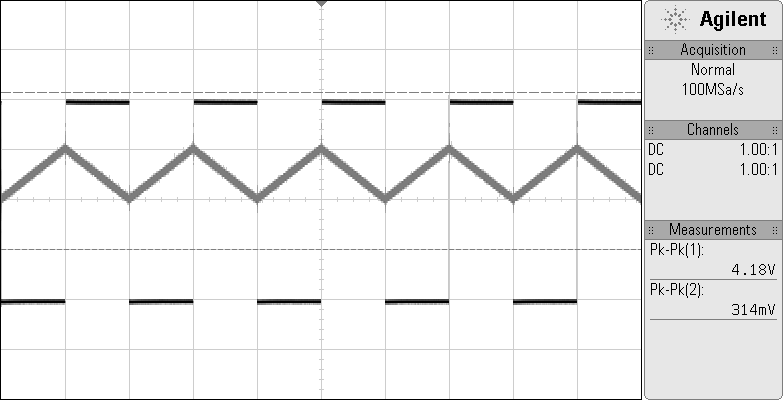
\includegraphics[width=\textwidth]{s10.png}
        \caption{Input: onda quadra -- Output: dente di sega}
        \label{fig:a1}
    \end{subfigure}
    \begin{subfigure}[t]{0.49\textwidth}
        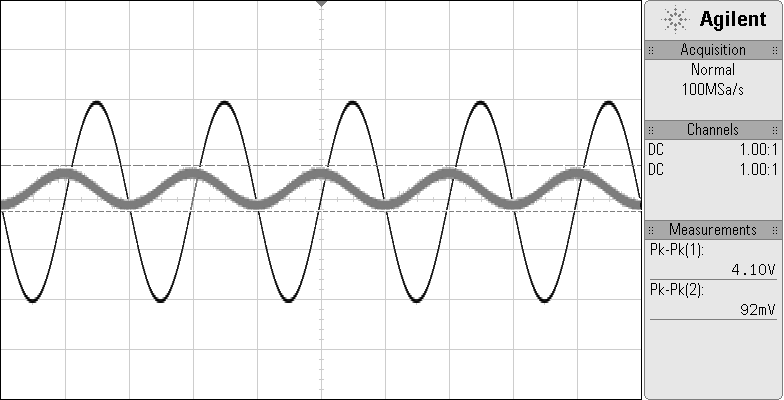
\includegraphics[width=\textwidth]{s11.png}
        \caption{Input: sinusoide -- Output: cosinusoide}
        \label{fig:a2}
    \end{subfigure}
    \caption{La figura mostra due esempi di funzionamento del circuito integratore. Tutte le figure
        sono state misurate con segnali a 1 kHz. Nel primo è stata fornita in ingresso
    un onda quadra ed il circuito risponde perfettamente generando delle rampe, mentre nel secondo abbiamo fornito una sinusoide
    e il circuito produce un coseno (si noti che i massimi e minimi dell'output sono nei punti di massima pendenza dell'input).
    L'output è indicato dalle linee grige. Si noti anche che l'output è un segnale molto debole se comparato con l'input
    (nelle misure a fianco è indicato dal valoe Pk-Pk(2)), poichè siamo a 1 kHz e la frequenza di taglio. Si noti che
    l'integratore è invertente.
    }
    \label{fig:iint}
\end{figure}

Abbiamo verificato la risposta del circuito al variare della frequenza. Essendo presente un capacitore
nella retroazione, il circuito si comporta come un filtro passa-basso. La resistenza $R_2$ serve ad evitare che a basse
frequenze la capacità apra il circuito. In pratica il circuito funziona bene tra pochi Hz e circa 160 Hz (frequenza di taglio
del filtro). Oltre 160 Hz il circuito funziona ancora ma il filtro attenue i segnali.

Inoltre abbiamo provato a rimuovere la resistenza di retroazione $R_2$, per vedere cosa sarebbe successo al circuito.
Il risultato è stato che l'output aveva un offset di 14.3 V a 1 kHz. Inoltre l'offset (come anche l'ampiezza del segnale
di output) è piccolo a basse frequenze, aumenta per frequenze di qualche migliaio di Hertz,
e poi torna a diminuire oltre i circa 20 kHz. Ad alte frequenze l'integratore non funziona bene.

\begin{figure}[b!]
    \centering
    \begin{subfigure}[t]{0.49\textwidth}
        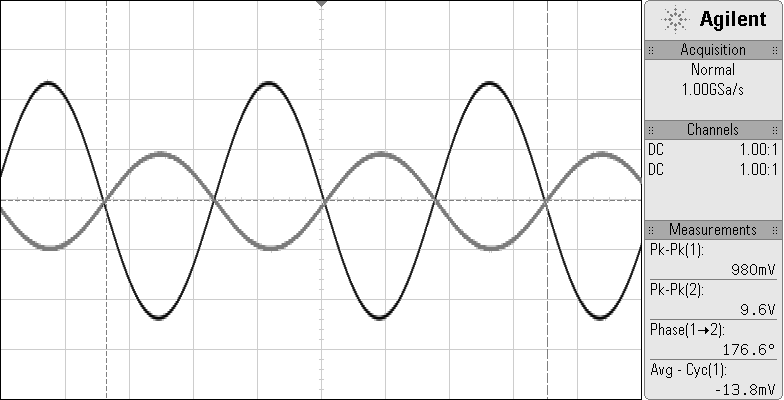
\includegraphics[width=\textwidth]{s12.png}
        \caption{Seno a 10 kHz}
        \label{fig:b1}
    \end{subfigure}
    \begin{subfigure}[t]{0.49\textwidth}
        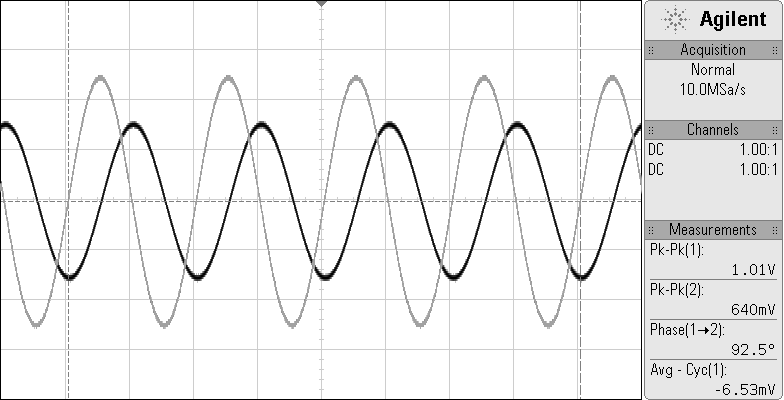
\includegraphics[width=\textwidth]{s13.png}
        \caption{Seno a 100 Hz}
        \label{fig:b2}
    \end{subfigure}
    \begin{subfigure}[t]{0.49\textwidth}
        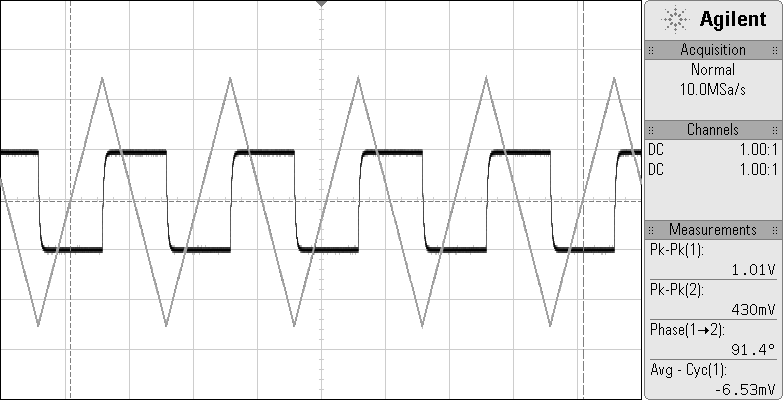
\includegraphics[width=\textwidth]{s14.png}
        \caption{Dente di sega a 100 Hz}
        \label{fig:b3}
    \end{subfigure}
    \begin{subfigure}[t]{0.49\textwidth}
        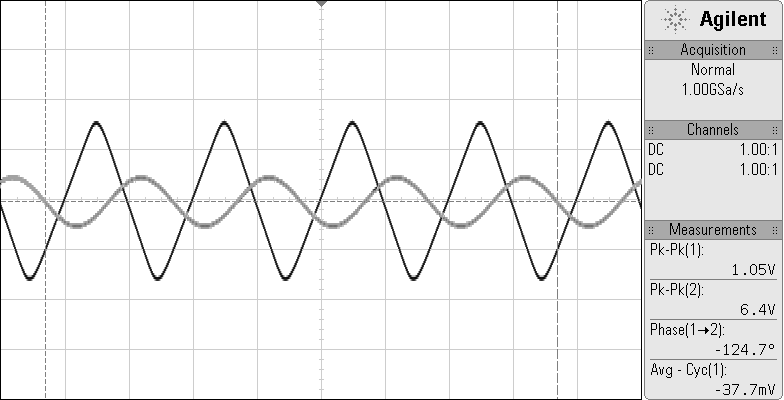
\includegraphics[width=\textwidth]{s16.png}
        \caption{Seno a 50 kHz}
        \label{fig:b4}
    \end{subfigure}
    \caption{La figura mostra il funzionamento del derivatore a varie frequenze e per varie funzioni in ingresso
        (input (1) in grigio).
        Nelle figure (b) e (c) il derivatore funziona perfettamente, anche se riduce il segnale in ingresso, poichè
        siamo a 100 Hz che è al disotto della frequenza di taglio del circuito. Aumentando la frequenza, come nell'immagine
        (a) si ottiene che il segnale è amplificato di circa 10 volte (il circuito si comporta come un
        amplificatore con guadagno G = 10 studiato all'inizio della relazione a causa delle resistenze). Tuttavia
        il derivatore sfasa l'output in maniera peculiare. Lo sfasamento implica che la deriva è errata. Aumentando ancora
        la frequenza (figura (d)) in guadagno diminuisce e il circuito si comporta in modo ancora più strano. Si noti che
        il derivatore è invertente.}
    \label{fig:scope}
\end{figure}

\subsection*{Circuito derivatore}

Per finire abbiamo montato un circuito derivatore, illustrato in Figura \ref{fig:diff}.
Le specifiche del circuito sono riportate in figura.
Lo scopo di questo circuito è quello di fornire in output un segnale $V\ped{out}$
che sia la derivata temporale del segnale in ingresso $V\ped{in}$. In formule si dovrebbe ottenere
che, se il circuito fosse ideale:

\begin{equation}
        V\ped{out}\,=\,-R_1C \cdot \frac{dV\ped{in}}{dt}
\end{equation}
%
dove con $R_1$ indichiamo la resistenza in serie al condensatore di capacità $C$ e
$V\ped{in}$ è il segnale in ingresso al circuito, variabile nel tempo.

Anche per questo circuito abbiamo voluto verificarne il corretto funzionamento, sfruttando l'oscilloscopio, osservando che $V\ped{out}$ sia effettivamente la derivata del segnale in ingresso $V\ped{in}$. Abbiamo quindi fornito in input vari segnali
tutti di ampiezza picco-picco 1.01 V. I risultati ottenuti sono illustrati in Figura \ref{fig:scope}.

In questo caso il circuito dovrebbe comportarsi come un filtro passa-alto con frequenza di taglio di circa 150 Hz.
Abbiamo quindi studiato l'andamento del guadagno in funzione
della frequenza, ottenendo il grafico in Figura \ref{fig:GGG}. Ad alte frequenze (sopra i 20 kHz) il circuito funziona male e
deriva in modo non corretto oltre a non amplificare esattamente come un filtro passa alto (il guadagno cala).
Questo ultimo fatto assieme ai valori dello sfasamento, che partono da circa 90$^\circ$ a 0 Hz, ci fa pensare a un filtro
passa-banda più che a un passa-alto. Non riusciamo a spiegarci questo fatto.

\begin{SCfigure}[1][h]
    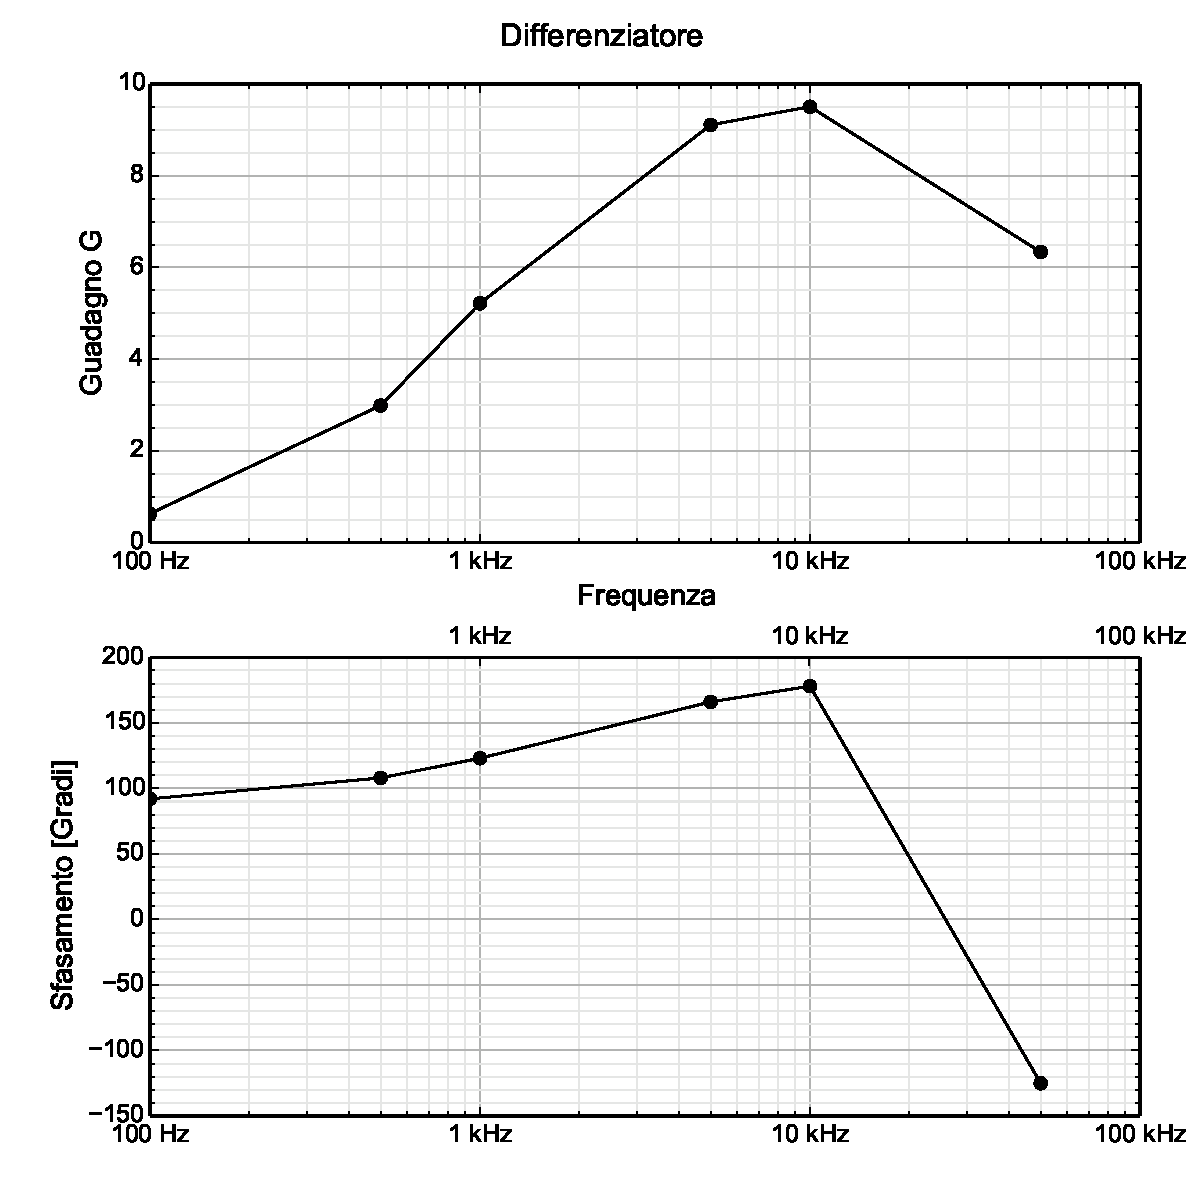
\includegraphics[width=0.75\textwidth]{diff.pdf}
    \caption{Il grafico mostra lo studio del differenziatore in funzione della frequenza.
        Abbiamo usato un segnale sinusoidale. Il circuito si comporta
        un po' come un filtro passa banda, partendo a 100 Hz con 90$^\circ$ di sfasamento rispetto al segnale in ingresso
        (in pratica deriva bene) ma attenuando il segnale. In seguito tra i 5 kHz e i 10 kHz il guadagno è massimo,
        ma il segnale viene sfasato fino a 180$^\circ$. Superando i 10 kHz, il guadagno cala, e lo sfasamento cambia
        improvvisamente segno. Purtroppo abbiamo raccolto troppi pochi dati per definire meglio l'andamento vicino al punto
        di cambio segno. Le incertezze sono della dimensione dei punti.}
    \label{fig:GGG}
\end{SCfigure}
